\documentclass[fleqn]{article}
\usepackage[UTF8]{ctex}
\usepackage{listings}
\usepackage{pdfpages}
\usepackage{color}
\usepackage[colorlinks,linkcolor=blue]{hyperref}
\usepackage{dashrule}
\usepackage{diagbox}
\usepackage[german]{babel}
\usepackage[T1]{fontenc}
\usepackage[latin1]{inputenc}
\usepackage{titlesec}
\usepackage{geometry}
\usepackage{qtree}
\usepackage{tikz}
\usepackage{amsmath}
\usepackage{amssymb}
\setcounter{secnumdepth}{0}
\usetikzlibrary{positioning}
\geometry{top=2.5cm, bottom=2.5cm}
\lstset{
 columns=fixed,       
 numbers=left,                                        % 在左侧显示行号
 numberstyle=\tiny\color{gray},                       % 设定行号格式
 frame=none,                                          % 不显示背景边框
 backgroundcolor=\color[RGB]{245,245,244},            % 设定背景颜色
 keywordstyle=\color[RGB]{40,40,255},                 % 设定关键字颜色
 numberstyle=\footnotesize\color{darkgray},           
 commentstyle=\it\color[RGB]{0,96,96},                % 设置代码注释的格式
 stringstyle=\rmfamily\slshape\color[RGB]{128,0,0},   % 设置字符串格式
 showstringspaces=false,                              % 不显示字符串中的空格
 language=c++,                                        % 设置语言
 breaklines,                                          % 自动换行
}

% \title{TU Chemnitz}

% \author{Dongze Yang}

\begin{document}

% \maketitle

\tableofcontents

\newpagestyle{main}{
    \sethead{}{}{CG1}
    \setfoot{}{\thepage}{}
    \headrule
    \footrule
}
\pagestyle{main}


\section{Übung 1 - Logikgatter, Amdahl'schesGesetz, Moore‘schesGesetz, Architekturen, Befehlsätze, Parallelität, Datenspeicherung}

\noindent\textbf{逻辑门,阿姆达尔定律,摩尔定律,体系结构,指令集,并行性,数据存储}
\\
\\
\noindent\textbf{1. 电路的真值表,与其名称}

\begin{center}
    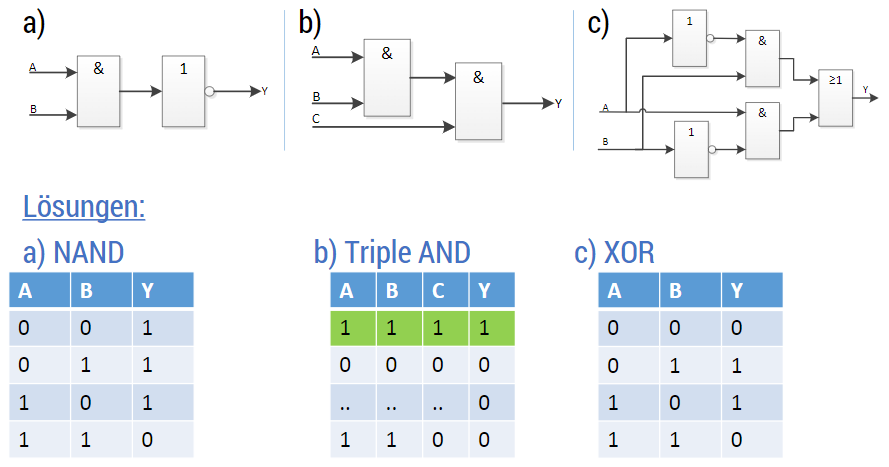
\includegraphics[scale=0.6]{1.png}
\end{center}

\noindent\textbf{2. Amdahl'sches Gesetz 阿姆达尔定律}

A: 3 Zeiteinheiten, B: 2 Zeiteinheiten, C: 5 Zeiteinheiten.

Optimierungsmöglichkeiten:

\indent\indent - A: 5 mal so schnell

\indent\indent - B: 10 mal so schnell

\indent\indent - C: 2 mal so schnell

Welche Optimierungsmöglichkeit bringt den größten Vorteil? 哪个优化选项带来最大优势?

\textbf{Ans: C}

Für A: 2.4 ZE ($3\times(1-\frac{1}{5})$), für B ZE ($2\times-\frac{1}{10}$), für C ZE ($5\times(1-\frac{1}{2})$)

\begin{center}
    \begin{tabular}{|c|c|c|c|c|}
        \hline
        &A&B&C&Summe\\
        \hline
        Zeiteinheiten T &3&2&5&10\\
        \hline
        Optimierung S&5&10&2&\\
        \hline
        Anteil P&0.3&0.2&0.5&1\\
        \hline
        \hline
        in \%&24&18&25&\\
        \hline
        Resultierende Zeit&7.6&8.2&7.5&\\
        \hline
        \hline
        Speedup S&1.31578947&1.2195122&1.33333333&\\
        \hline
    \end{tabular}
\end{center}

\noindent\textbf{3. Moore'sches Gesetz 摩尔定律}

Die Anzahl von Transistoren auf einem Chip beträgt 5 Mrd. . Nach Moores Law, wieviele Transistoren hat ein ähnlich dimensionierter Chip in 3 Jahren? Ist diese Transistorzahl realistisch?

芯片上的晶体管数量为50亿个。 根据摩尔定律,在三年内,一个类似大小的芯片有多少个晶体管? 这样数量的晶体管现实吗?

\textbf{Ans:} 20 Mrd..

Nach Moores Law verdoppelt sich die Anzahl der Transistoren auf einem Chip alle 18 Monate.

根据摩尔定律,芯片上的晶体管数量每18个月翻一番。

Dies stößt zunehmend an physikalische Grenzen, ab welchen keine kleineren Transistoren entworfen werden könnenMoore‘schesGesetz.

这越来越多地遇到了物理极限,超过该极限就无法根据摩尔定律设计更小的晶体管。
\\
\\
\noindent\textbf{4. Architekturen 架构}

Worin unterscheiden sich Havard-Architektur und Von-Neumann-Architektur? Was sind die jeweiligen Vor-und Nachteile?

哈佛架构和冯·诺依曼架构有什么区别? 各自的优点和缺点是什么?

\textbf{Havard-Architektur}
 
Getrennter Speicher für Programm und Daten 程序和数据的独立存储器

Gleichzeitig, aber mehr Aufwand (Bus, Speicher) =  Kosten 同时,但更多的消耗(总线,内存)=成本

\textbf{Von-Neumann-Architektur}

Gleicher Speicher für Programm und Daten 程序和数据的内存相同

Weniger Aufwand, Befehl-ODER Datenzugriff 减少工作量,命令或数据访问
\\
\\
\noindent\textbf{5. Befehlsätze 指令集}

Worin unterscheiden sich RISCund CISC? RISC和CISC有什么区别?

\textbf{ReducedInstructionSet Computer –RISC}

verwenden einen einfachen Befehlssatz, dessen Befehle sehr effizient abgearbeitet werden können

使用简单的指令集,可以非常有效地处理其指令

\textbf{Complex Instruction Set Computer –CISC}

haben hingegen einen komplexen Befehlssatz 但是,指令集比较复杂

Kann das gleiche mit weniger Schritten, aberi.d.R. langsamer als RISC

可以用更少的步骤做同样的事情,但是通常 比RISC慢

\noindent\textbf{6. Parallelität 并行性}

Womit wird Parallelität auf Befehlsebene umgesetzt? Beschreiben sie (grob) ein Beispiel.

在命令级别如何实现并行性? 大致描述一个例子.

\textbf{Ans:} Pipeline

\indent\indent Mehr Durchsatz, Befehle pro Zeit. 更高的吞吐量,每次命令

\indent\indent Befehlsabhängigeitensind problematisch (zw. Befehlen). 命令依赖关系存在问题(命令之间)

\indent\indent Z.B.: Mehrere Einheiten (S1= Abrufen, S2=Dekodieren, S3=Operation, etc). 例如:几个单位(S1 =检索,S2 =解码,S3 =操作等)

\begin{center}
    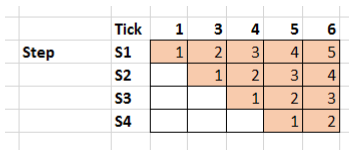
\includegraphics[scale=0.6]{2.png}
\end{center}

\noindent\textbf{7. Datenspeicherung 数据存储}

- Welche Varianten der Datenspeicherung gibt es? (Stichwort Bytereihenfolge)

有哪些类型的数据存储?(关键字字节顺序)

\textbf{Ans:} Big Endian/Little EndianHöchstes/niedrigstes Bit zuerst. 大端/小端 $\rightarrow$ 高/低Bit优先

\begin{center}
    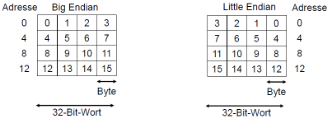
\includegraphics[scale=0.6]{3.png}
\end{center}

- Beschreiben sie grob (Pseudocode) ein Programm, um 粗略地描述(伪码)程序

\qquad $\circ$ BE nach LE zu überführen 将BE转移到LE

\qquad $\circ$ LE nach BE zu überführen 将LE转移到BE

\textbf{Ans:} Beides der gleiche Vorgang

\qquad Bsp: 

\qquad \qquad $For (x=0, x<=length-1),x++$

\qquad \qquad \qquad $New(x)=Old(length-1-x);$
\\
\\
\indent- Was repräsentiert der Hammingabstandzwischen zwei Codewörtern? Berechnen sie diesen für 1001 0010 und 1000 0011. Welche Paritätsbits haben diese beiden Codewörter? Wievielezusätzliche Korrekturbits sind für Codewörter der Länge 8 notwendig?

两个代码字之间的汉明距离代表什么? 为1001 0010和1000 0011计算此值。这两个代码字具有哪些奇偶校验位? 长度为8的代码字需要多少个其他校正位?

\textbf{Ans:} 

\qquad a) Anzahl sich unterscheidender Bitstellen. Hier im Beispiel: 2. 不同位置的数量,此处为2.

\qquad b) Paritätsbits sind beide 1 (ungerade Anzahl 1-Bits) 奇偶校验位均为1(奇数为1位)

\qquad c) $(m+r+1)\leq 2^r$, wobei m = Länge und r = Anzahl Prüfbits $\rightarrow$ 4 Prüfbits. m为长度,r为校验位数
\\
\\
\indent-Wie werden Fehlerkorrekturbits zur Erkennung von Einzelbitfehlern genutzt? Beschreiben sie eine Möglichkeit für das Codewort1010 (3 Prüfbits)

纠错位如何用于检测单个位错误?描述码字1010(3个校验位)的可能性。

\begin{center}
    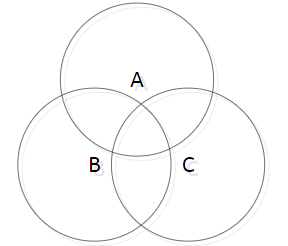
\includegraphics[scale=0.6]{4.png}
\end{center}

\textbf{Ans:} Bits B1 bis B4, Prüfbits A B C $\rightarrow$ Wort B1 B2 B3 B4 A B C

\qquad \qquad B1 = A + B + C\qquad B2 = A + B\qquad  B3 = B + C\qquad B4 = A + C

\begin{center}
    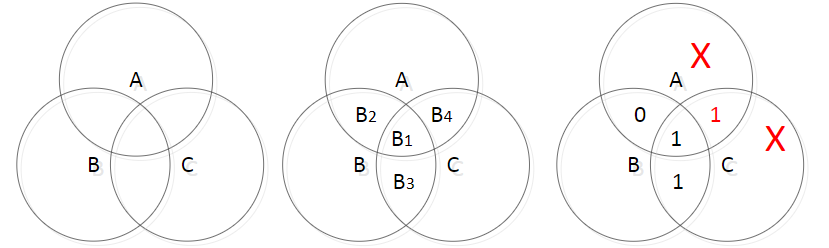
\includegraphics[scale=0.5]{5.png}
\end{center}















































































\end{document}